\chapter{\IfLanguageName{dutch}{Proof of concept}{Proof of concept}}
\label{ch:proof-of-concept}

\section{\IfLanguageName{dutch}{Opstelling proof of concept}{Setup proof of concept}}
De proof of concept (zie figuur:\ref{fig:opstelling_arduino}) is opgesteld uit:
\begin{itemize}
	\item Arduino MKR GSM 1400 Cellular Kit (80.35 euro);
	\item Arduino MKR GPS Shield (41.75 euro);
	\item Lithium Ion Polymeer Accu - 3.7V 2500mAh (25.9 euro).
\end{itemize}
De totale kost van de proof of concept komt neer op \textbf{148 euro}. Naast de lage kost heeft de proof of concept de mogelijkheid om zelf volledig geconfigureerd te worden. De configuratie is gebeurd in de editor van Arduino zelf. Het script moest in staat zijn om de volgende functies uit te voeren:
\begin{itemize}
	\item De locatie bepalen aan de hand van GPS;
	\item De locatie bepalen aan de hand van AGPS;
	\item De locatie doorsturen naar een REST API aan de hand van een POST request (JSON).
\end{itemize}
Het script is zelf ontwikkeld en staat opensource op \href{https://github.com/IndyVC/bap-arduino}{een github repository}. In het script werd gebruik gemaakt van allerlei libraries om het traceren mogelijk te maken.
Er werd gebruik gemaakt van:
\begin{itemize}
	\item \href{https://github.com/arduino-libraries/ArduinoHttpClient}{ArduinoHttpClient}: voor het versturen van data via POST requests;
	\item \href{https://github.com/arduino-libraries/MKRGSM}{MKRGSM}: voor het gebruik van mobiele data;
	\item \href{https://github.com/bblanchon/ArduinoJson}{ArduinoJson}: het mogelijk maken om makkelijk een JSON body op te vullen;
	\item \href{https://github.com/arduino-libraries/Arduino_MKRGPS}{ArduinoMKRGPS}: voor het bepalen van de locatie via GPS.
\end{itemize}
De proof of concept maakt gebruik van een simkaart (zie figuur: \ref{fig:simkaart}) om online data te kunnen versturen. 
\begin{figure}
	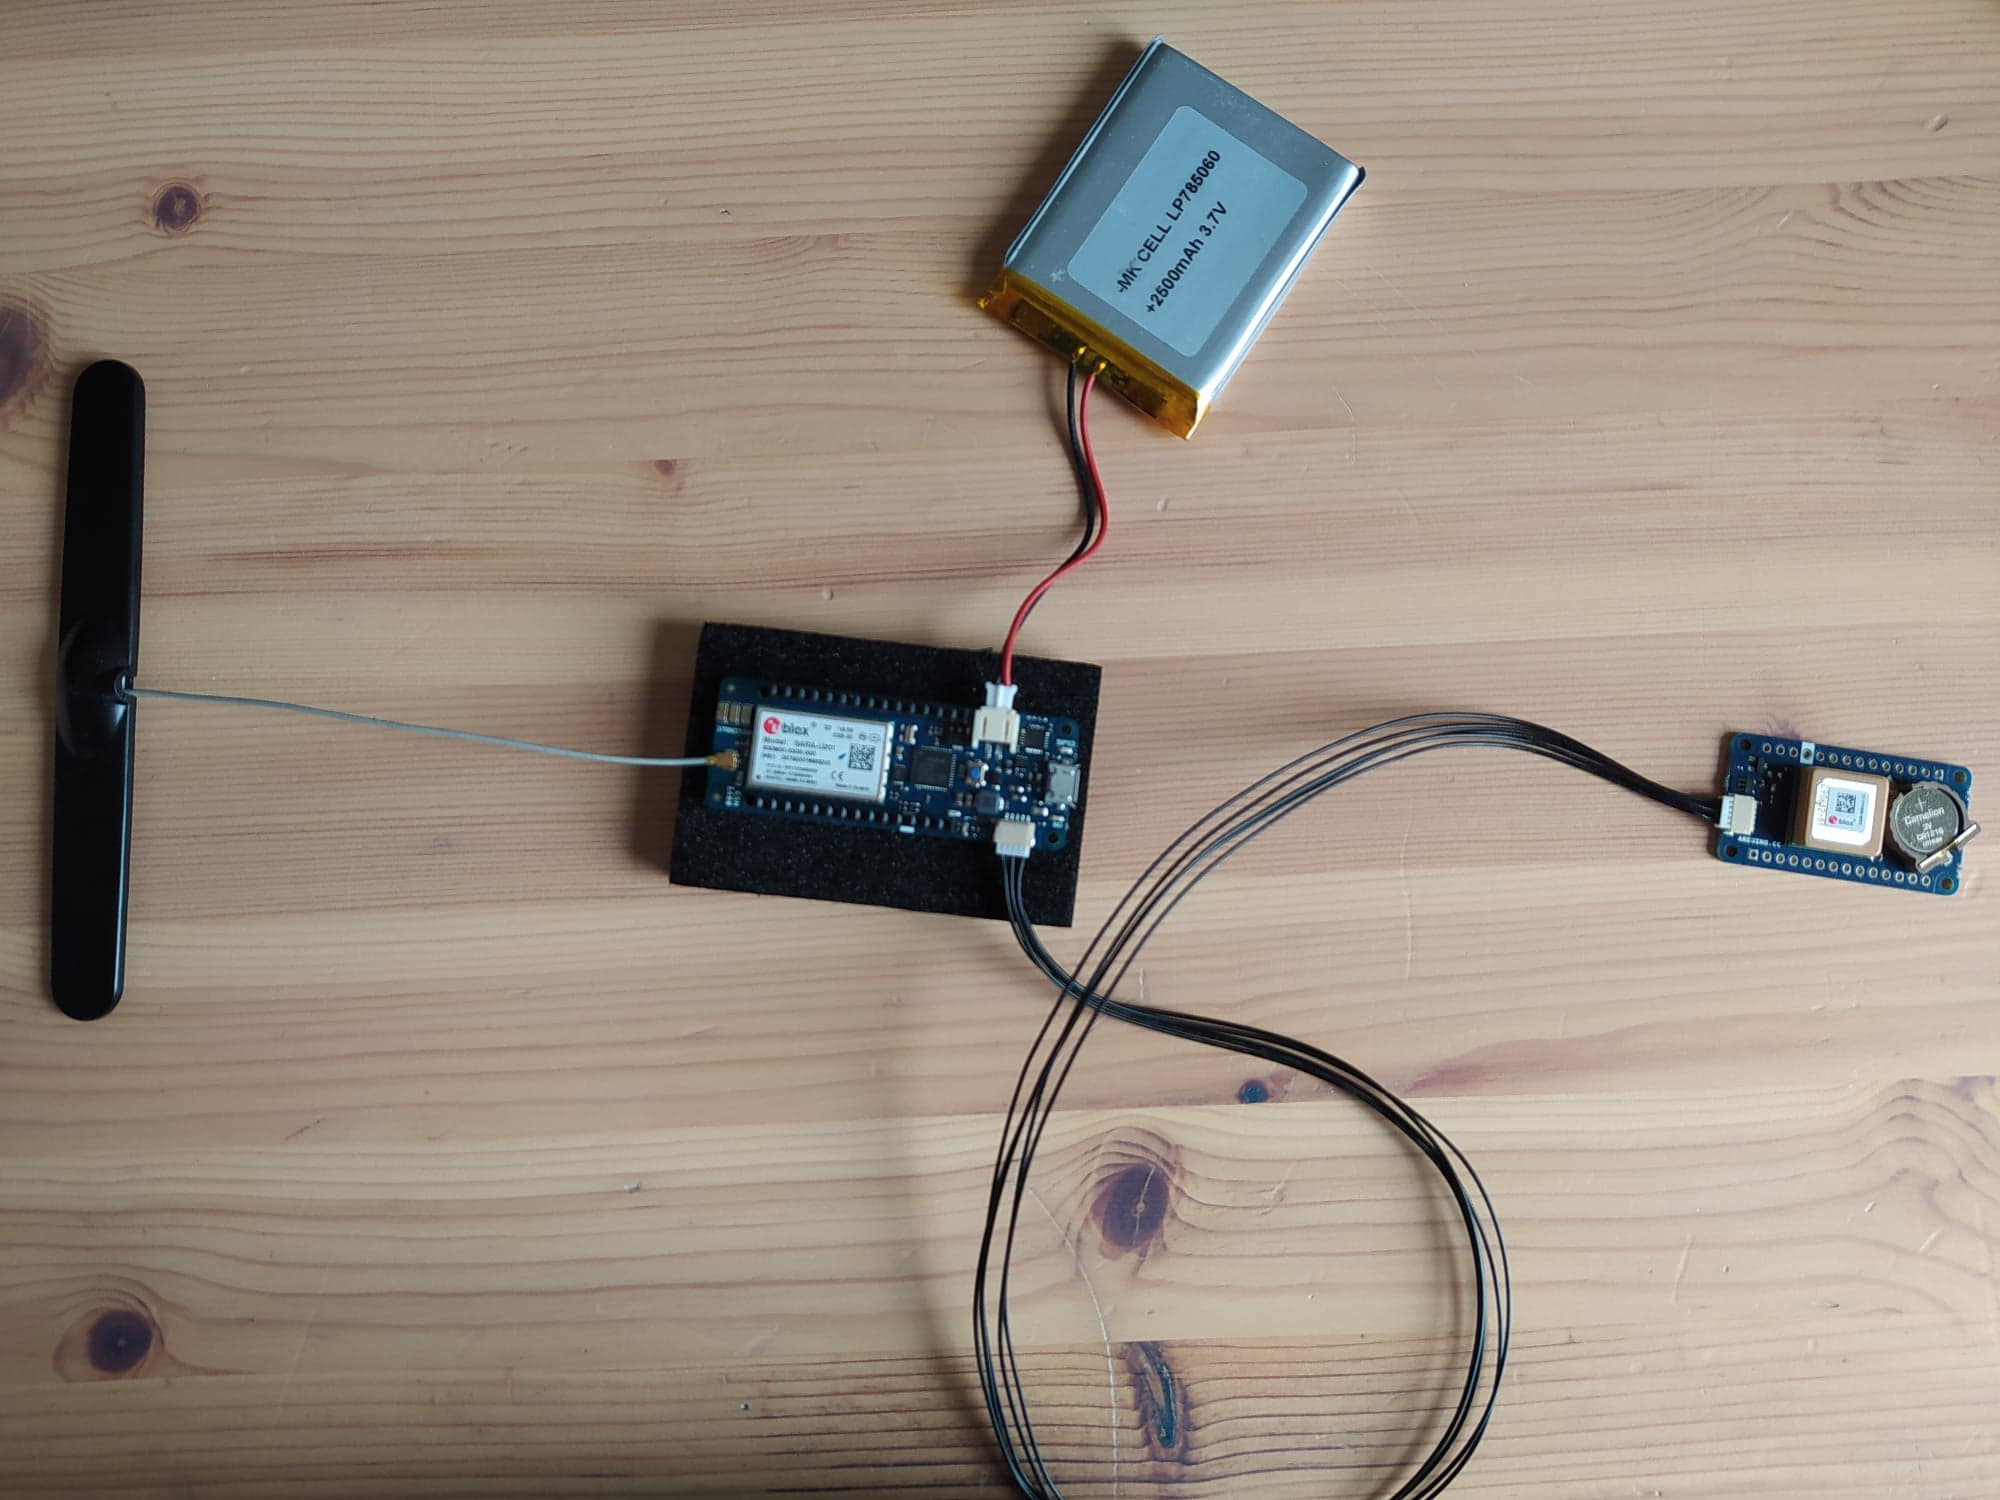
\includegraphics[width=\textwidth,height=\textheight,keepaspectratio]{opstelling_arduino.jpg}
	\caption{opstelling proof of concept}
	\label{fig:opstelling_arduino}
\end{figure}
\begin{figure}
	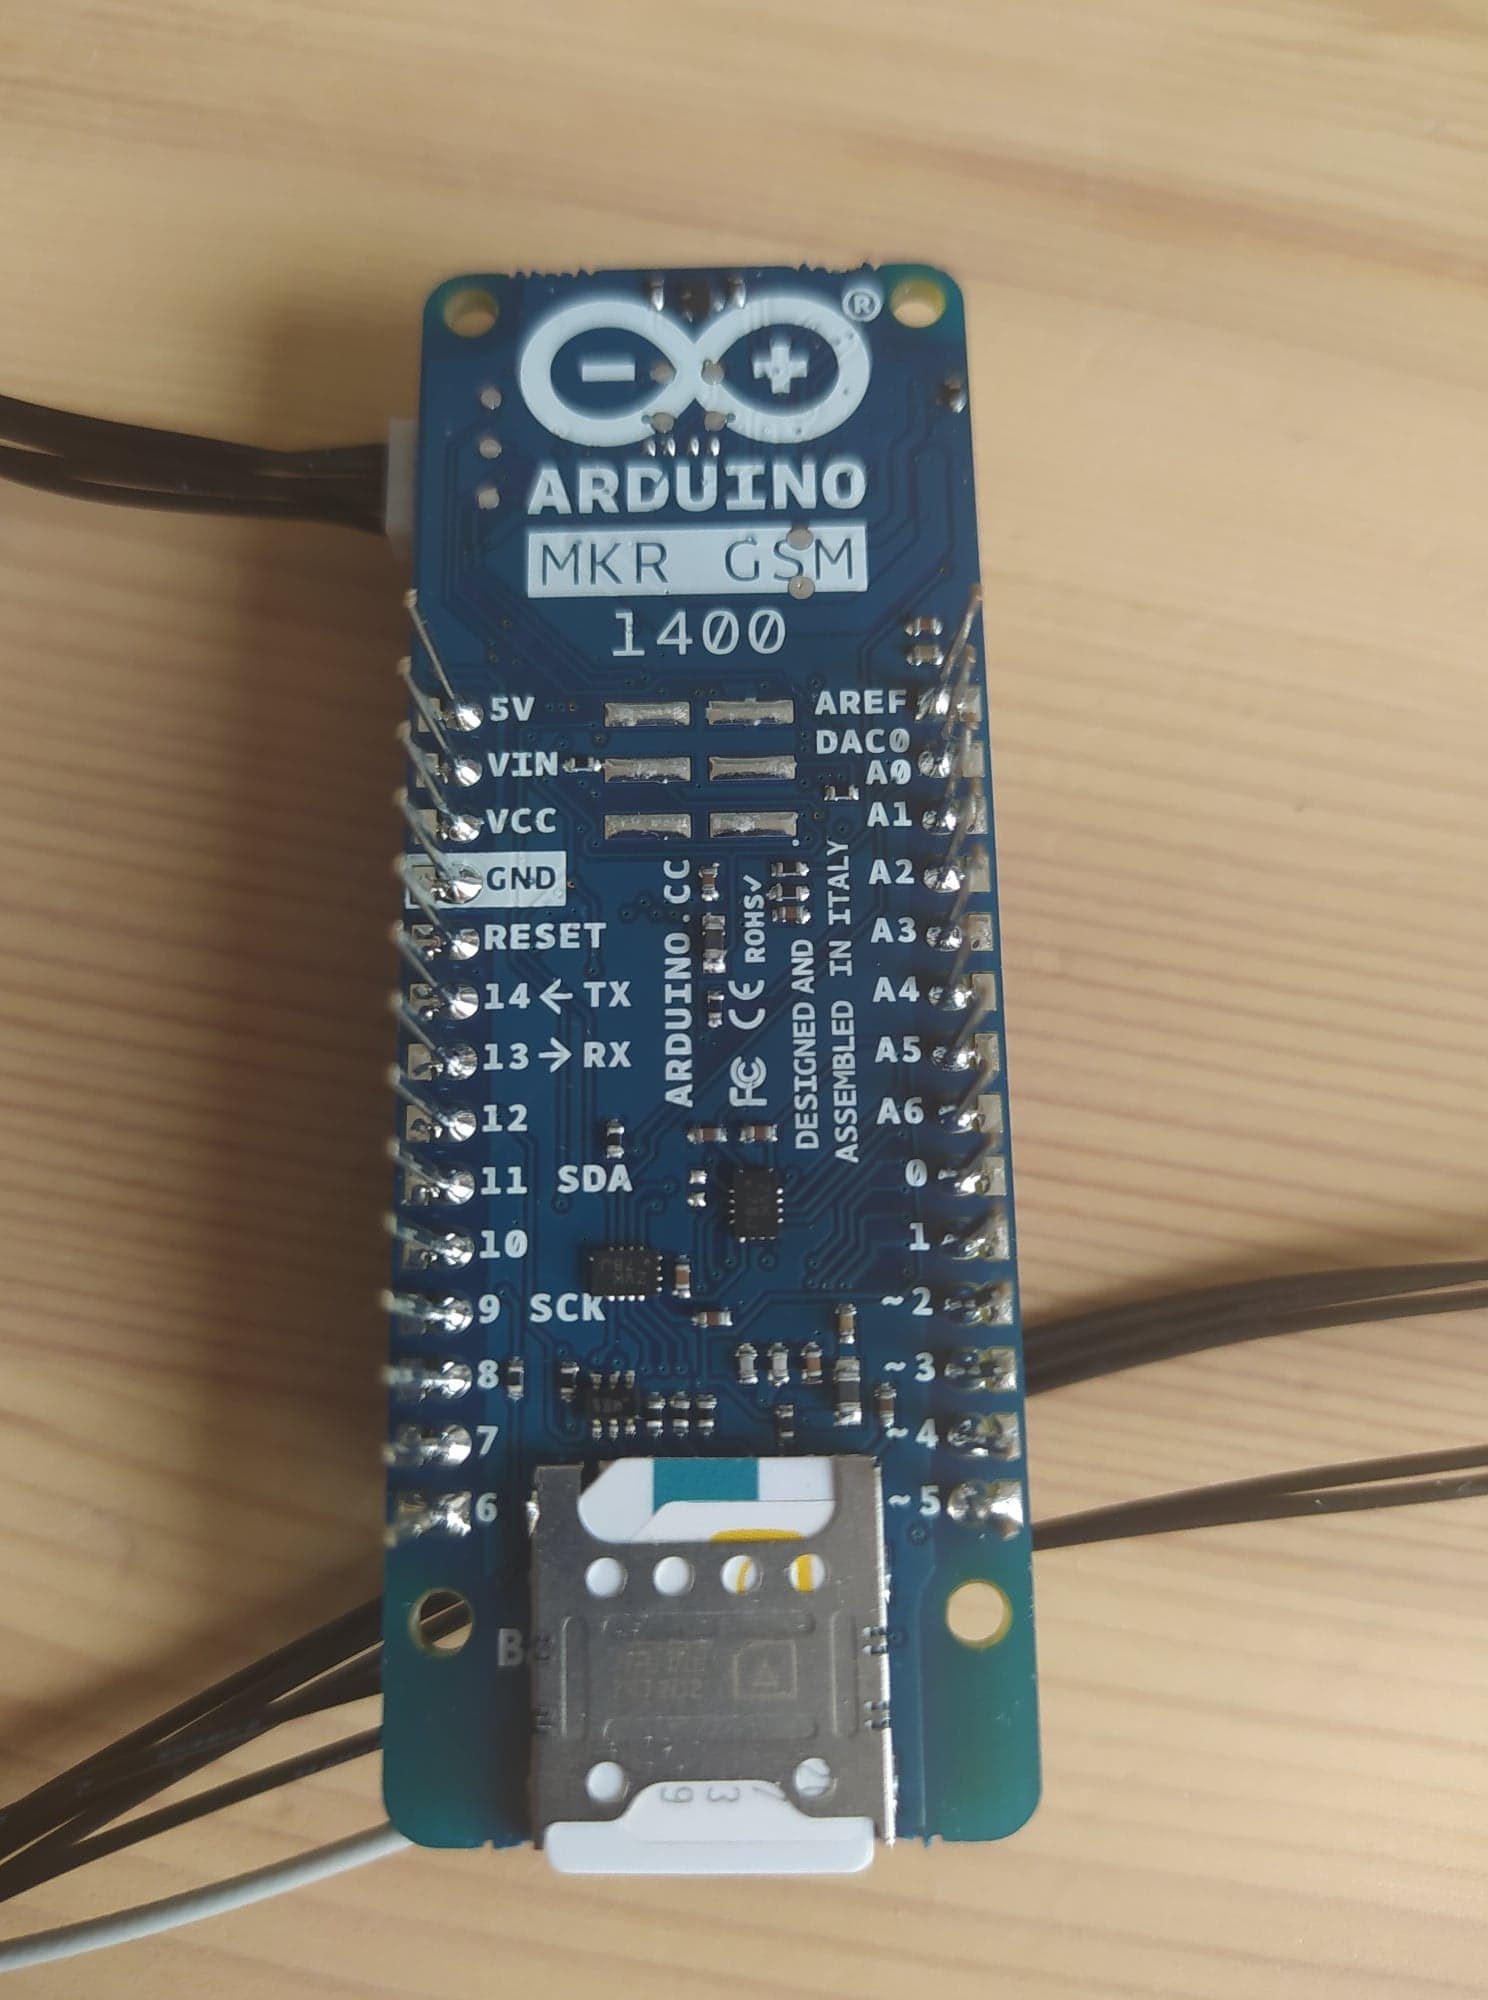
\includegraphics[width=\textwidth,height=\textheight,keepaspectratio]{simkaart.jpg}
	\caption{Simkaart}
	\label{fig:simkaart}
\end{figure}

\section{\IfLanguageName{dutch}{Waterdichte casing}{Waterproof casing}}
TODO: NOG AAN TE VULLEN